\documentclass[ima, 20pt, portrait, plainboxedsections]{sciposter}

% Packages
\usepackage[english]{babel}
\usepackage[latin1]{inputenc}
\usepackage{times}
\usepackage{amsmath,amssymb}
\usepackage{multicol}
\usepackage{mathtools}
\usepackage{epstopdf}

\usepackage{authblk}


\usepackage[section]{placeins}
\usepackage{booktabs}

\usepackage{graphicx}
\usepackage{algorithmic}

% TEMPLATE PARAMETERS
\setlength{\parskip}{0.002\textheight}
\newcommand{\imsize}{0.49\columnwidth}
\definecolor{BoxCol}{rgb}{0.4,0.4,0.4}
\definecolor{SectionCol}{rgb}{1,1,1}
\renewcommand{\titlesize}{\Huge}
\renewcommand{\sectionsize}{\Large}
\setmargins[2cm]

% HEADER
\setlength{\titlewidth}{0.5\textwidth}
\setlength{\logowidth}{0.25\textwidth}

\leftlogo[0.9]{kaust_cuq_logo_left}
%\rightlogo[0.95]{kaust_cuq_logo_right}
%\leftlogo[0.7]{kaust}

% Theorems
\newtheorem{thm}{Theorem}[section]
%\newtheorem{proof}[thm]{Proof}
%\newtheorem{lemma}[thm]{Lemma}
\newtheorem{rem}[thm]{Remark}
\newtheorem{cor}[thm]{Corollary}
\newtheorem{ex}[thm]{Example}
\newtheorem{assu}[thm]{Assumption}
\newtheorem{alg}[thm]{Algorithm}
\newtheorem{defn}[thm]{Definition}

% Commands
\newcommand{\ceil}[1]{\lceil {#1} \rceil}
\newcommand{\seqof}[3]{(#1)_{#2}^{#3}}

\newcommand{\ssa}{\text{SSA}}
\newcommand{\hyb}{\text{Hyb}}
\newcommand{\MNRM}{\text{MNRM}}
\newcommand{\TL}{\text{TL}}
\newcommand{\ML}{\text{ML}}
\newcommand{\Li}{L^{\text{int}}}
\newcommand{\Ls}{L_c^{\text{exp}}}
\newcommand{\Lc}{L_c^{\text{imp}}}


%\newcommand{\NSSA}{N_{\ssa}}
\newcommand{\NSSAKone}{N_{\ssa,K1}}
\newcommand{\NSSAKtwo}{N_{\ssa,K1'}}

%\newcommand{\NMNRMKone}{N_{\MNRM,K1}}
%\newcommand{\NMNRMKtwo}{N_{\MNRM,K2}}
%\newcommand{\NMNRMKoneC}{N_{\MNRM,K1}^{(c)}}
%\newcommand{\NMNRMKtwoC}{N_{\MNRM,K2}^{(c)}}

\newcommand{\NMNRMKone}{N_{K1}}
\newcommand{\NMNRMKtwo}{N_{K2}}
\newcommand{\NMNRMKoneC}{N_{K1}^{(c)}}
\newcommand{\NMNRMKtwoC}{N_{K2}^{(c)}}

\newcommand{\NMNRM}{N_{\MNRM}}
\newcommand{\NMNRMC}{N_{\MNRM}^{(c)}}
%\newcommand{\NMNRMP}{N_{{\MNRM}^*}}

\newcommand{\NSSAP}{N_{{\ssa}^*}}
\newcommand{\NTL}{N_{\TL}}
\newcommand{\NTLP}{N_{{\TL}^*}}
\newcommand{\NTLC}{N_{\TL}^{(c)}}
%\newcommand{\NTLF}{\dbar N_{\TL}}

\newcommand{\EE}{\mathcal{E}}

\newcommand{\WE}{\EE_I}
\newcommand{\WEC}[1]{\EE_{I,#1}}
\newcommand{\WEH}[1]{\hat \EE_{I,#1}}
\newcommand{\WSSA}{\text{Cost}_{\ssa}}
\newcommand{\WHYB}{\text{Cost}_{\hyb}}


\newcommand{\avg}[2]{\mathcal{A}\left(#1;#2\right)}
%\newcommand{\SD}[2]{\mathcal{S}(#1;#2)}
\newcommand{\svar}[2]{\mathcal{S}^2\left(#1;#2\right)}

\newcommand{\dbar}[1]{\Bar{\Bar{#1}}}

\newcommand{\ie}{\emph{i.e.}}
\newcommand{\eg}{\emph{e.g.}}
\newcommand{\cf}{\emph{cf.}}
\newcommand{\ud}{\mathrm{d}}
\newcommand{\prob}[1]{\mathrm{P}\left(#1\right)}
\newcommand{\expt}[1]{\mathrm{E}\left[#1\right]}
\newcommand{\expth}[1]{\hat{\mathrm{E}}\left[#1\right]}

\newcommand{\var}[1]{\mathrm{Var}\left[#1\right]}
\newcommand{\cov}[2]{\mathrm{Cov}\left[#1, #2\right]}
\newcommand{\norm}[1]{\left\|#1\right\|}
\newcommand{\abs}[1]{\left|#1\right|}
\newcommand{\rset}{\mathbb{R}}
\newcommand{\nset}{\mathbb{N}}
\newcommand{\zset}{\mathbb{Z}}
\newcommand{\JAC}{\mathbb{J}}
\newcommand{\one}{\mathbf{1}}
\newcommand{\poisson}[1]{\mathcal{P}\left(#1\right)}
\newcommand{\normal}[1]{\mathcal{N}\left(#1\right)}
\newcommand{\binomial}[1]{\mathcal{B}\left(#1\right)}
\newcommand{\Ordo}[1]{{\mathcal{O}}\left(#1\right)}
\newcommand{\OrdoP}[1]{{\mathcal{O}_P}\left(#1\right)}
\newcommand{\ordo}[1]{{o}\left(#1\right)}
\newcommand{\abstr}[1]{\begin{abstract}#1\end{abstract}}
\newcommand{\thx}[1]{\thanks{#1}}
\newcommand{\red}[1]{{\color{red}#1}}
\newcommand{\blue}[1]{{\color{blue}#1}}
\newcommand{\green}[1]{{\color{magenta}#1}}

\newcommand{\latt}{\mbox{$\zset_+^d$}}


%Alvaro's notations

\newcommand{\indicator}[1]{\mathbf{1}_{#1}} 

\newcommand{\PERIOD}{.}
\newcommand{\COMMA}{,}

% Removed this command since it does not work properly with spacing
%\newcommand{\ChB}{{Chernoff bound }}
\newcommand{\LP}{\left(}
\newcommand{\RP}{\right)}

\newcommand{\LPe}{\left.}
\newcommand{\RPe}{\right.}

%\newcommand{\SEP}{\biggm|}
\newcommand{\SEP}{\, \big| \,}
\newcommand{\BX}{\bar X(t)}
\newcommand{\BXi}{\bar X_i(t)}
\newcommand{\BXitau}{\bar X_i(t{+}\tau)}

\newcommand{\sj}{\sum_{j=1}^J}

\newcommand{\Qi}{Q_i(t,\tau_i)}
\newcommand{\lji}{a_j(\bar X(t))\tau_i}
\newcommand{\Yj}{Y_j\left( a_j(\bar X(t))\tau_i \right)}
\newcommand{\ldi}{\log(\delta_i)}
\newcommand{\taui}{\tau_i(s)}
\newcommand{\DEN}[1]{- a_0 \LP \bar X(t) \RP +  \sj a_j(\bar X(t))e^{-#1\, \nu_{ji}}}
\newcommand{\aj}{ a_j(\bar X(t))}

\newcommand{\anu}{\sj \aj \nu_{ji}}
%\newcommand{\anu2}{\sj \aj (\nu_{ji})^2}
\newcommand{\tsi}{\tilde{s}_i}
\newcommand{\hs}{\hat{s}}
%\newcommand{\tti1}{\tilde{t}_{i,1}} 
\newcommand{\az}{a_0(\bar X(t))}
\newcommand{\dnux}{\delta_i^{\,\nu_{ji}/{\BXi}}}

\newcommand{\bj}{b_{ji}(\bar X(t))}
\newcommand{\mE}[1]{\mathcal{E}_{#1}}
\newcommand{\mV}[1]{\mathcal{V}_{#1}}
\newcommand{\hmV}[1]{\hat{\mathcal{V}}_{#1}}

\newcommand{\orden}{\alpha}

%Pedro's notations
\newcommand{\X}[1]{\bar X(t_{#1})}
\newcommand{\ti}[1]{t_{#1}}
%\newcommand{\iff}{\Leftrightarrow}

\newcommand{\algorithmfootnote}[2][\footnotesize]{%
  \let\old@algocf@finish\@algocf@finish% Store algorithm finish macro
  \def\@algocf@finish{\old@algocf@finish% Update finish macro to insert "footnote"
    \leavevmode\rlap{\begin{minipage}{\linewidth}
    #1#2
    \end{minipage}}%
  }%
}
%new command for switch case algo
% New definitions
%\algnewcommand\algorithmicswitch{\textbf{switch}}
%\algnewcommand\algorithmiccase{\textbf{case}}
%\algnewcommand\algorithmicassert{\texttt{assert}}
%\algnewcommand\Assert[1]{\State \algorithmicassert(#1)}%
%
%% New "environments"
%\algdef{SE}[SWITCH]{Switch}{EndSwitch}[1]{\algorithmicswitch\ #1\ \algorithmicdo}{\algorithmicend\ \algorithmicswitch}%
%\algdef{SE}[CASE]{Case}{EndCase}[1]{\algorithmiccase\ #1}{\algorithmicend\ \algorithmiccase}%
%\algtext*{EndSwitch}%
%\algtext*{EndCase}%

%%% Local Variables: 
%%% mode: latex
%%% TeX-master: "main_new"
%%% End: 


\newcommand{\subcaption}[1]% %1 = text
{\refstepcounter{subfig}%
	\par\vskip\abovecaptionskip
	\centerline{\textbf{(\alph{subfig})} #1}%
	\vskip\belowcaptionskip\par}

% create subfigure environment
\def\subfigure{\let\oldcaption=\caption
	\let\caption=\subcaption
	\minipage}
\def\endsubfigure{\endminipage
	\let\caption=\oldcaption}


% POSTER CONTENT

\title{Hierarchical adaptive sparse  grids and Quasi Monte Carlo for option pricing under the rough Bergomi model}

%\author{Christian Bayer\thanks{
% Weierstrass Institute for Applied Analysis and Stochastics (WIAS),
% Berlin, Germany.}
%        \and Chiheb Ben Hammouda\thanks{King Abdullah University of Science and Technology (KAUST), Computer, Electrical and Mathematical Sciences \& Engineering Division (CEMSE), Thuwal $23955-6900$, Saudi Arabia ({\tt chiheb.benhammouda@kaust.edu.sa}).} 
%\and  Raul Tempone\thanks{King Abdullah University of Science and Technology (KAUST), Computer, Electrical and Mathematical Sciences \& Engineering Division (CEMSE), Thuwal $23955-6900$, Saudi Arabia ({\tt raul.tempone@kaust.edu.sa}).} \thanks{Alexander von Humboldt Professor in Mathematics for Uncertainty Quantification, RWTH Aachen University, Germany.}}

%\author{Christian Bayer, Chiheb Ben Hammouda  and Raul Tempone}
%\institute{King Abdullah University of Science and Technology (KAUST) , Weierstrass Institute for Applied Analysis and Stochastics (WIAS)}

\author[1]{Christian Bayer}
\author[2]{Chiheb Ben Hammouda}
\author[3]{Raul Tempone}
\affil[1]{Weierstrass Institute for Applied Analysis and Stochastics (WIAS), Berlin, Germany.}
\affil[2]{King Abdullah University of Science and Technology (KAUST), Thuwal, Saudi Arabia}
\affil[3]{RWTH Aachen University, Germany.}
\setcounter{Maxaffil}{0}
\renewcommand\Affilfont{\normalsize\normalfont}

%\email{   \{chiheb.benhammouda,  raul.tempone \}@kaust.edu.sa}

\begin{document}

\maketitle

\begin{multicols}{3}

\section*{Abstract} 
The \red{rough Bergomi (rBergomi) model}, introduced in  \cite{bayer2016pricing}, is a promising rough volatility model in quantitative finance.  In the absence of analytical European option pricing methods for the model, and due to \red{the non-Markovian nature of the fractional driver}, the prevalent option is to use Monte Carlo (MC) simulation for pricing. Despite recent advances in the MC method in this context, pricing under the rBergomi model is still a time-consuming task. To overcome this issue, \red{we design a novel,  alternative, hierarchical approach, based on i) adaptive sparse grids quadrature (ASGQ)}, specifically using the same construction in \cite{haji2016multi}, and \red{ii) Quasi Monte Carlo (QMC)}. Both techniques are coupled with \red{Brownian bridge} construction and \red{Richardson extrapolation}. By uncovering the available regularity,  our hierarchical methods demonstrates \red{substantial computational gains with respect to the standard MC method}, when reaching a sufficiently small error tolerance in the price estimates across different parameter constellations, even for very small values of the Hurst  parameter.
%-------------
\section*{Rough Volatility}
\begin{figure}[H]
 \begin{center}
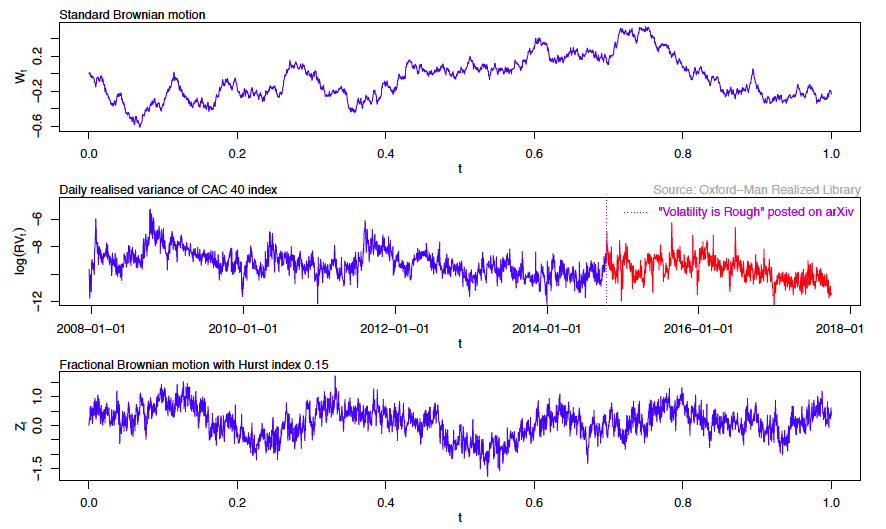
\includegraphics[scale=0.83]{vol_rough}
 \end{center}
\end{figure}
\section*{The rough Bergomi Model \cite{bayer2016pricing}}
This model, under a pricing measure, is given by
\begin{equation}
\begin{cases}
	dS_t &= \sqrt{v_t} S_t dZ_t,\\
v_t &= \blue{\xi_0}(t) \exp\left( \blue{\eta} \widetilde{W}_t^{\blue{H}} - \frac{1}{2} \blue{\eta}^2 t^{2\blue{H}} \right),\\
	Z_t&:=\blue{\rho}	W^1_t+ \bar{\rho}W^\perp_t \equiv \blue{\rho} W^1+\sqrt{1-\blue{\rho}^2} W^\perp,
\end{cases}
\end{equation}
\begin{itemize}
	\item $(W^1,W^\perp)$: two independent standard Brownian motions
	\item $\widetilde{W}^\blue{H} $ is \red{Riemann-Liouville process},  defined by
	\begin{align*}
	\widetilde{W}_t^{\blue{H}} &= \int_0^t K^{\blue{H}}(t-s) dW_s^1, \quad t \ge 0, \\ 	K^{\blue{H}}(t-s) &= \sqrt{2\blue{H}} (t-s)^{\blue{H} - 1/2},\quad \forall \: 0 \le s \le t.
	\end{align*}
	\item $\blue{H} \in(0,1/2]$ ($H=1/2$ for Brownian motion): controls the \red{roughness} of paths, , $\blue{\rho} \in [-1,1]$  and  $\blue{\eta}>0$.
	\item $t \mapsto \blue{\xi}_0(t)$: forward variance curve, known at time $0$.
\end{itemize}
\section*{Challenges}
\begin{itemize}
\item \textbf{Numerically:}
	\begin{itemize}
		\item The model is \red{non-affine} and \red{non-Markovian} $\Rightarrow$ Standard numerical methods (PDEs, characteristic functions) seem inapplicable.
		\item The only prevalent pricing method for mere
		\red{vanilla options} is \red{Monte Carlo} \cite{bayer2016pricing,bayer2017regularity,mccrickerd2018turbocharging}, still a \red{time consuming task}.
		
\item 	Discretization methods have \red{poor behavior of the strong error}, that is the convergence rate is of order of $\blue{H} \in[0,1/2]$ \cite{neuenkirch2016order} $\Rightarrow$ Variance reduction methods, such as MLMC, are inefficient for \red{very small values} of $\blue{H}$.
	\end{itemize}

\item \textbf{Theoretically:} 
\begin{itemize}
\item No proper weak error analysis done in the rough volatility
context.
\end{itemize}
\end{itemize}
\section*{Contributions}
\begin{enumerate}		
		\item We design an \red{alternative hierarchical efficient pricing method} based on:
		\begin{enumerate}
			\item[i)] \red{Analytic smoothing}  to uncover available regularity.
			\item[ii)] Approximating the option price using a \red{deterministic quadrature method (ASGQ and QMC)} coupled with \red{Brownian bridges} and \red{Richardson Extrapolation}.
		\end{enumerate} 
	\item Our \red{hierarchical} methods demonstrate \red{substantial} computational gains with respect to the standard MC method, assuming a \red{sufficiently small relative error tolerance} in the price estimates, even for \red{small values of}, $\blue{H}$.		
		\end{enumerate}
\section*{On the Choice of the Simulation Scheme}
\begin{figure}[h!]
	\centering
	\begin{subfigure}{.52\textwidth}
		\centering
		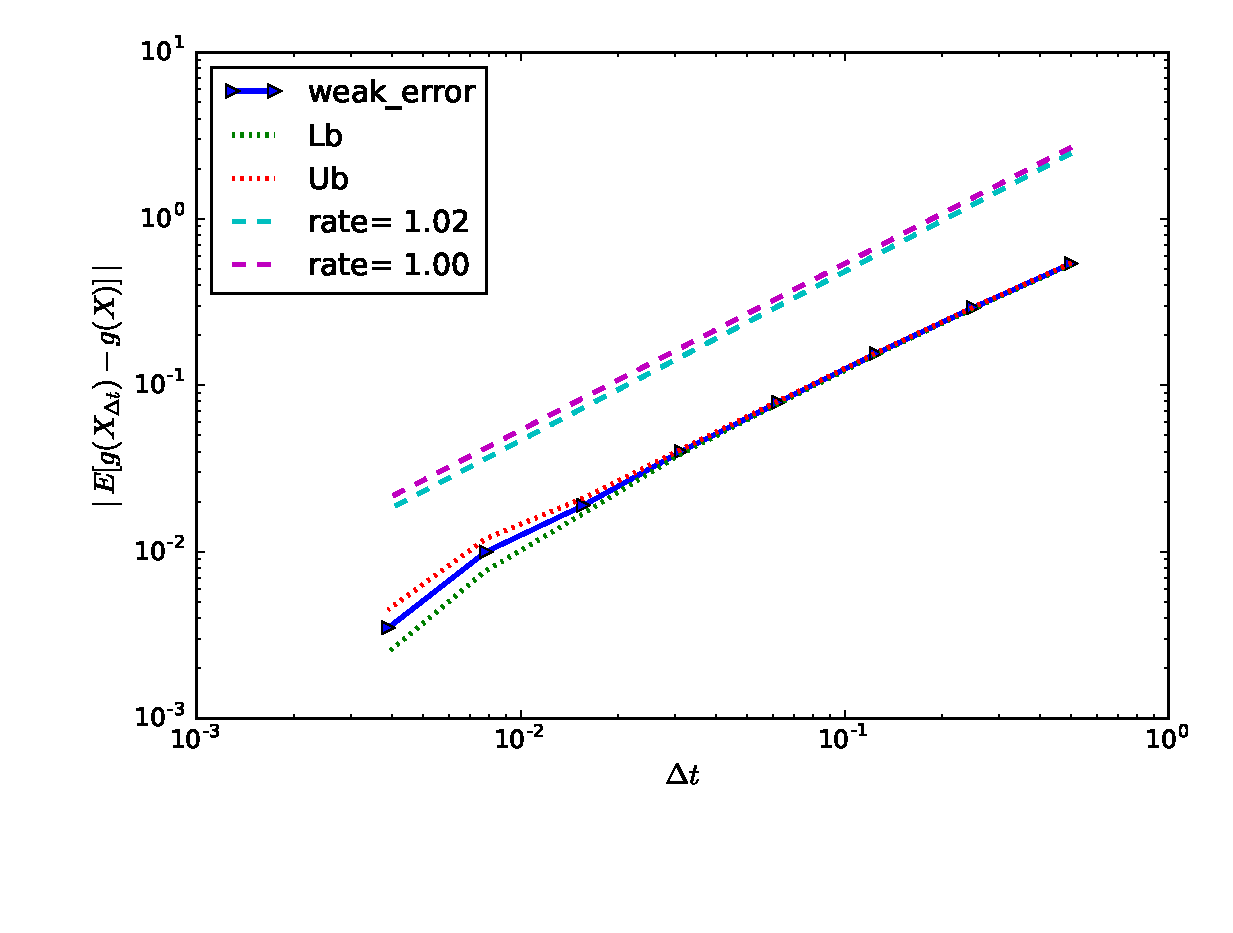
\includegraphics[width=1\linewidth]{./rBergomi_weak_error_rates/without_richardson/H_007/weak_convergence_order_Bergomi_H_007_K_1_M_4_10_6_CI_relative_hybrid_non_hierarchical_non_parallel_asymptotic}
		\caption{}
		\label{fig:set1_weak_rate_hybrid}
	\end{subfigure}%
	\begin{subfigure}{.52\textwidth}
		\centering
		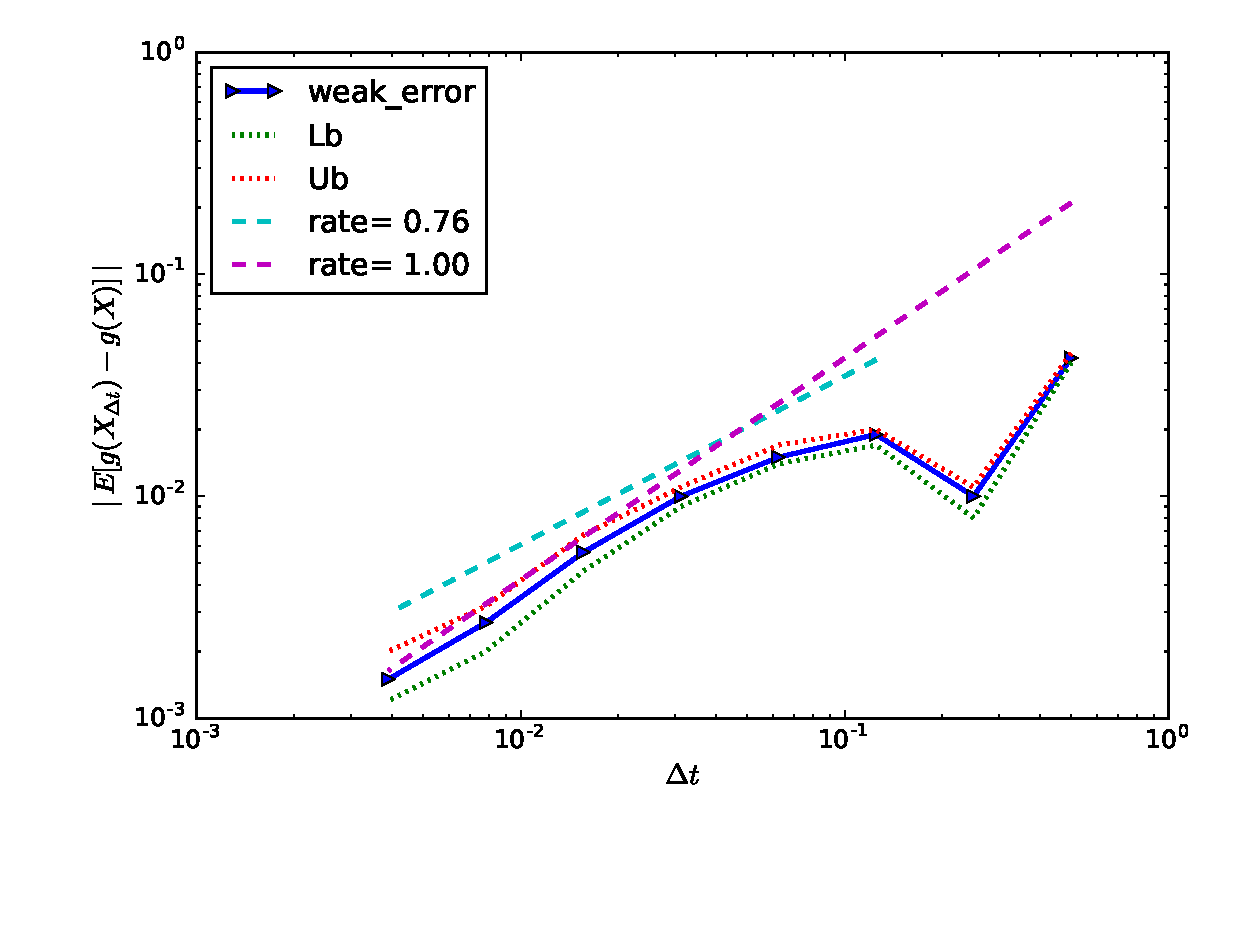
\includegraphics[width=1\linewidth]{./rBergomi_weak_error_cholesky/weak_convergence_order_Bergomi_H_007_K_1_M_4_10_6_CI_relative_cholesky_non_hierarchical_non_parallel_asymptotic}
		\caption{}
		\label{fig:set1_weak_rate_exact}
	\end{subfigure}
	\caption{The convergence of the weak error $\mathcal{E}_B$, using MC with $6 \times 10^6$ samples, for \red{Set $1$ parameter in Table \ref{table:Reference solution, using MC with $500$ time steps, of Call option price under rBergomi model, for different parameter constellation.}}. The upper and lower bounds are $95\%$ confidence intervals. a) With \red{the hybrid scheme}  b) With \red{the exact scheme}.}
	\label{fig:Weak_rate_set1_set_2_without_rich_hyb+chol}
\end{figure}
\section*{The Hybrid Scheme \cite{bennedsen2017hybrid}}
\begin{align*}
	\widetilde{W}_t^{\blue{H}} &= \int_0^t K^{\blue{H}}(t-s) dW_s^1, \quad t \ge 0, \\ 	K^{\blue{H}}(t-s) &= \sqrt{2\blue{H}} (t-s)^{\blue{H} - 1/2},\quad \forall \: 0 \le s \le t. 
	\end{align*}
\begin{itemize}
\item 	The hybrid scheme \red{discretizes} the  $\widetilde{W}^\blue{H}$ process into \red{Wiener integrals of power functions and a Riemann sum}, appearing from approximating the kernel by power functions near the origin and step functions elsewhere.
\begin{align*}
\widetilde{W}^H_{\frac{i}{N}} \approx \overline{W}^H_{\frac{i}{N}}&= \sqrt{2H} \left(  W^2_i+\sum_{k=2}^{i} \left(\frac{b_k}{N}\right)^{H-\frac{1}{2}} \left(W_{\frac{i-(k-1)}{N}}^1-W_{\frac{i-k}{N}}^1\right)\right)\COMMA
\end{align*}
\begin{itemize}
\item $N$ is the number of time steps 
\item $\{W^{2}_j\}_{j=1}^N$: \red{Artificially introduced} $N$ Gaussian random variables that are used for left-rule points in the hybrid scheme.
\item $b_k=\left(\frac{k^{H+\frac{1}{2}}-(k-1)^{H+\frac{1}{2} }}{H+\frac{1}{2}}\right)^{\frac{1}{H-\frac{1}{2}}}.$
\end{itemize}
\end{itemize}
\section*{The rough Bergomi Model: Analytic Smoothing}
\begin{align}\label{BS_formula_rbergomi}
C_{RB}\left( T, K \right) &= E\left[ \left(S_T - K \right)^+ \right]  \nonumber\\
&=\expt{\expt{(S_T-K)^+ \mid \sigma(W^1(t) ,t \le T)}}\nonumber \\
&=E\left[C_{BS}\left( \blue{S_0} = \operatorname{exp}\left(\rho \int_0^T \sqrt{v_t} dW_t^1 - \frac{1}{2}
\rho^2 \int_0^T v_t dt\right), \right. \right.\nonumber\\
&\quad \quad \quad \left.\left.\ \blue{k} = K , \ \blue{\sigma^2} = (1-\rho^2)
\int_0^T v_t dt \right) \right]\nonumber\\
&\approx \int_{\rset^{2\red{N}}} C_{BS} \left(G(\mathbf{w}^{(1)},\mathbf{w}^{(2)})\right) \rho_{\red{N}}(\mathbf{w}^{(1)})  \rho_{\red{N}}(\mathbf{w}^{(2)}) d\mathbf{w}^{(1)} d\mathbf{w}^{(2)}\nonumber\\
&=C_{RB}^N \COMMA
\end{align}
\begin{itemize}
\item $C_{\text{BS}}(\blue{S_0},\blue{k},\blue{\sigma^2})$ denotes the Black-Scholes call price, for initial spot price $\blue{S_0}$, strike price $\blue{k}$, and volatility $\blue{\sigma^2}$.
\item $G$ maps $2N$ independent standard Gaussian random inputs to the parameters fed to Black-Scholes formula.
\item $\rho_{\red{N}}$: the multivariate Gaussian density, $\red{N}$: number of time steps.
\end{itemize} 
%\section*{Sparse Grids I}
%\textbf{\blue{Goal:}} Given  $F: \rset^d \rightarrow \rset$ and a multi-index $\boldsymbol{\beta} \in \mathbb{N}^d_{+}$, \red{approximate}
%\begin{displaymath} \expt{F} \approx Q^{m(\boldsymbol{\beta})}[F], \end{displaymath} 
%where $Q^{m(\boldsymbol{\beta})}$ a Cartesian quadrature grid with $m(\beta_n)$ points along $y_n$.
%
%\textbf{\blue{Idea:}} Denote $Q^{m(\boldsymbol{\beta})}[F]=F_{\boldsymbol{\beta}}$ and introduce the \red{first difference} 
%
%\begin{equation}
%\begin{aligned}
%\Delta_i F_{\boldsymbol{\beta}} \left\{ \begin{array}{rcr}
%F_{\boldsymbol{\beta}} - F_{\boldsymbol{\beta}-e_i}, & \text{ if } \beta_i>1  \\ 
%F_{\boldsymbol{\beta}}  & \text{ if } \beta_i=1  \end{array} \right. \\
%\end{aligned}
%\end{equation}
%
%where $e_i$ denotes the $i$th $d$-dimensional unit vector, and \red{mixed difference operators}
%
%\begin{equation}
%\Delta [F_{\boldsymbol{\beta}}]= \otimes_{i = 1}^{d} \Delta_iF_{\boldsymbol{\beta}}
%\end{equation}
\section*{Sparse Grids}
A quadrature estimate of $E[F]$ is
\begin{equation}\label{eq:Quadrature_estimator}
\mathcal{M}_{\mathcal{I_{\ell}}}[F]=\sum_{\boldsymbol{\beta} \in \mathcal{I}_{\ell}} \Delta [F_{\boldsymbol{\beta}}]\COMMA \quad (\Delta:  \text{mixed difference operator})
\end{equation}
\begin{itemize}
\item \red{Product approach}: $\mathcal{I}_{\ell}=\{ \max\{\beta_1,\dots,\beta_d \} \le \ell;\: \boldsymbol{\beta} \in \mathbb{N}^d_{+} \} $
\item \red{Regular SG}: $ \mathcal{I}_{\ell}=\{  \mid \boldsymbol{\beta} \mid_1 \le \ell+d-1; \: \boldsymbol{\beta} \in \mathbb{N}^d_{+} \} $

%		\begin{figure}
%		\centering
%		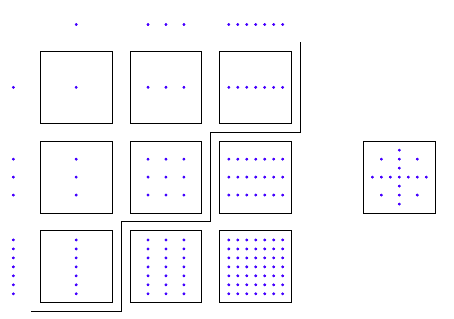
\includegraphics[scale=0.5]{sparse_grids}
%		\vspace{0.1cm}
%		\caption{Left are product grids $\Delta_{\beta_1} \otimes \Delta_{\beta_2}$ for $1 \le \beta_1, \beta_2 \le 3$. Right is the corresponding SG construction.}
%		\label{fig:vol_rough}
%	\end{figure}
%	\vspace{0.3cm}
\item \red{ASGQ} based on same construction as in \cite{haji2016multi}: $\mathcal{I}_{\ell}=\blue{\mathcal{I}^{\text{ASGQ}}}$.
\end{itemize}
\section*{ASGQ in Practice}
\begin{itemize}
		\item The construction of \blue{$\mathcal{I}^{\text{ASGQ}}$} is done by profit thresholding
		
 \begin{equation*}
 \blue{\mathcal{I}^{\text{ASGQ}}}=\{\boldsymbol{\beta} \in \mathbb{N}^d_{+}: \blue{P_{\boldsymbol{\beta}}}	 \ge \overline{T}\}.
 \end{equation*}
 	\item \textbf{Profit of a hierarchical surplus} \blue{$P_{\boldsymbol{\beta}}= \frac{\abs{\Delta E_{\boldsymbol{\beta}}}}{\Delta\mathcal{W}_{\boldsymbol{\beta}}}$}.
 \item \textbf{Error contribution}:  \blue{ $\Delta E_{\boldsymbol{\beta}} = \abs{\mathcal{M}^{\mathcal{I} \cup \{\boldsymbol{\beta}\}}-\mathcal{M}^{\mathcal{I}}}$}.
 %how much the error decreases if the operator $\Delta[F_{\boldsymbol{\beta}}]$ is added to \blue{$\mathcal{M}_{\mathcal{I}}[F]$
 \item \textbf{Work contribution}:  \blue{$ 		\Delta \mathcal{W}_{\boldsymbol{\beta}} = \text{Work}[\mathcal{M}^{\mathcal{I} \cup \{\boldsymbol{\beta}\}}]-\text{Work}[\mathcal{M}^{\mathcal{I}}]$}
	\end{itemize}
\begin{figure}
	\centering
	\begin{subfigure}{0.3\textwidth}
		\centering
		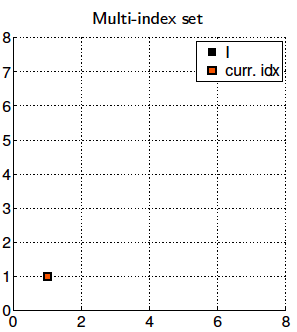
\includegraphics[width=0.9\textwidth]{./MISC_construction/1}
		\caption{}
	\end{subfigure}\hfil
	\begin{subfigure}{0.3\textwidth}
		\centering
		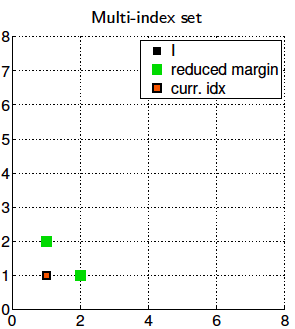
\includegraphics[width=0.9\textwidth]{./MISC_construction/2}
		\caption{}
	\end{subfigure}\hfil
	\begin{subfigure}{0.3\textwidth}
		\centering
		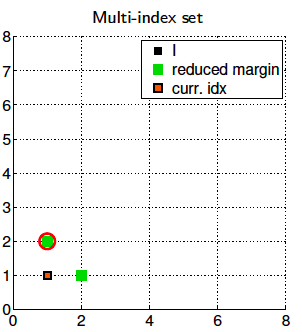
\includegraphics[width=0.9\textwidth]{./MISC_construction/3}
		\caption{}
	\end{subfigure}\hfil
	\medskip
\begin{subfigure}{0.3\textwidth}
	\centering
	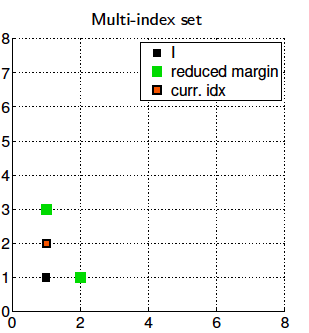
\includegraphics[width=0.9\textwidth]{./MISC_construction/4}
	\caption{}
\end{subfigure}\hfil
\begin{subfigure}{0.3\textwidth}
	\centering
	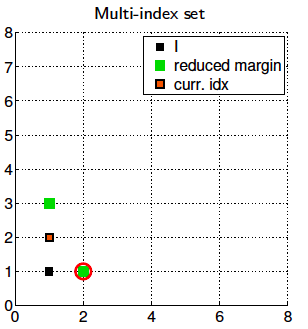
\includegraphics[width=0.9\textwidth]{./MISC_construction/5}
	\caption{}
\end{subfigure}\hfil
\begin{subfigure}{0.3\textwidth}
	\centering
	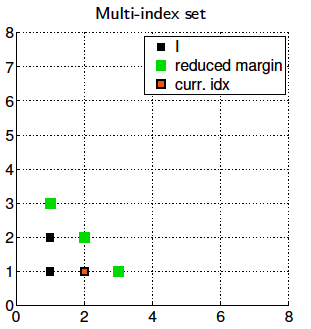
\includegraphics[width=0.9\textwidth]{./MISC_construction/6}
	\caption{}
\end{subfigure}%
	\caption{Construction of the index set for ASGQ method. \red{A posteriori, adaptive construction}: Given an index set $\mathcal{I}_k$, compute the profits of the neighbor indices and select the most profitable one.}
\end{figure}



\section*{Error Comparison}
$\red{\mathcal{E}_{\text{tot}}}$: the total error of approximating the  expectation in \eqref{BS_formula_rbergomi} 
\begin{itemize}
	\item When using ASGQ estimator, $Q_N$
	\begin{align}\label{eq:total_error_ASGQ}
	\red{\mathcal{E}_{\text{tot}}} & \le \abs{C_{\text{RB}}-C_{\text{RB}}^N}+\abs{C_{\text{RB}}^N-Q_{N}} \le \green{\mathcal{E}_B(N)}+ \blue{\mathcal{E}_Q(\text{TOL}_{\text{ASGQ}},N)},
	\end{align}
where  $\mathcal{E}_Q$ is the quadrature error, $\green{\mathcal{E}_B}$  is the bias, $\blue{\text{TOL}_{\text{ASGQ}}}$ is a user selected tolerance for ASGQ method.
\item When using randomized QMC or MC estimator,   $Q^{\text{MC (QMC)}}_N$
		\begin{align}\label{eq:total_error_MC}
	\red{\mathcal{E}_{\text{tot}}} & \le \abs{C_{\text{RB}}-C_{\text{RB}}^N}+\abs{C_{\text{RB}}^N-Q^{\text{MC (QMC)}}_N} \le \green{\mathcal{E}_B(N)}+ \blue{\mathcal{E}_{S}(M,N)},
	\end{align}
	where  $\blue{\mathcal{E}_S}$ is the statistical error, $M$ is the number of samples used for MC or randomized QMC method.
	\item The number of samples, $M^{\text{QMC}}$ and $M^{\text{MC}}$, are chosen so that  the statistical errors of QMC, $\mathcal{E}_{S,\text{QMC}}(M^{\text{QMC}})$, and MC, $\mathcal{E}_{S,\text{MC}}(M^{\text{MC}})$, satisfy
	\begin{align}\label{optimal_number_samples}
	\blue{\mathcal{E}_{S,\text{QMC}}(M^{\text{QMC}})}=\blue{\mathcal{E}_{S,\text{MC}}(M^{\text{MC}})}= \green{\mathcal{E}_B(N)}=\frac{\red{\mathcal{E}_{\text{tot}}}}{2}\COMMA
	\end{align}
\end{itemize}


\section*{Numerical Experiments}
\begin{table}[!h]
\begin{small}
	\centering
\caption{Reference solution, using MC with $500$ time steps and number of samples, $M=8 \times 10^6$, of call option price under the rough Bergomi model, for different parameter constellations.  The numbers between parentheses correspond to the statistical errors estimates.}
\label{table:Reference solution, using MC with $500$ time steps, of Call option price under rBergomi model, for different parameter constellation.}
	\begin{tabular}{l*{2}{c}r}
	\toprule[1.5pt]
		\textbf{Parameters}            & \textbf{Reference solution}    \\
	\hline
		
		Set $1$:	$H=0.07, K=1,S_0=1, T=1, \rho=-0.9, \eta=1.9,\xi_0=0.235^2$   & $\underset{(5.6e-05)}{0.0791}$  \\	
		
		Set $2$:	$H=0.02, K=1, S_0=1, T=1,\rho=-0.7, \eta=0.4,\xi_0=0.1$   & $\underset{(9.0e-05)}{0.1246}$  \\
		Set $3$:	$H=0.02, K=0.8,S_0=1,T=1, \rho=-0.7, \eta=0.4,\xi_0=0.1$   & $\underset{(5.4e-05)}{0.2412}$  \\
		Set $4$:	$H=0.02, K=1.2,S_0=1,T=1, \rho=-0.7, \eta=0.4,\xi_0=0.1$   & $\underset{(8.0e-05)}{0.0570}$  \\
	\bottomrule[1.25pt]
	\end{tabular}
	\end{small}
\end{table}

\begin{itemize}
\item The first set is the  \red{closest to the empirical findings} \cite{gatheral2018volatility,bennedsen2016decoupling}, suggesting that $\blue{H} \approx 0.1$. The choice of values $\blue{\nu}= 1.9$ and $\blue{\rho}=-0.9$ is justified by \cite{bayer2016pricing}.

\item  For the remaining three sets, we wanted to test the potential of our method for a \red{very rough case}, where variance reduction methods are inefficient.
\end{itemize}
\section*{Relative Errors and Computational Gains of the Different Methods.}
\begin{table}[!h]
	\centering
	\caption{ In this table, we highlight the computational gains achieved by ASGQ and QMC over MC method to meet a certain error tolerance. We note that the ratios are computed \red{for the best configuration with Richardson extrapolation for each method}.}
	\begin{small}
		\begin{tabular}{l*{4}{c}r}
			\toprule[1.5pt]
			\textbf{Parameter set}              &  \textbf{Total relative error}  & \textbf{CPU time ratio $\left(\text{MC}/ \text{ASGQ} \right)$} & \textbf{CPU time ratio  $\left(\text{MC}/ \text{QMC} \right)$}\\
			\hline
			Set $1$  &  $1\%$&  $ 15$ &  $10$\\	
			
			\hline
		Set $2$    &  $0.2\%$&  $21.5$ &  $73.2$\\		
			\hline
		Set $3$   &  $0.4\%$&  $26.7$ &  $21.3$\\	
			\hline
		Set $4$ &  $2\%$&  $5$ &  $10$\\	
			\bottomrule[1.25pt]
		\end{tabular}
	\end{small}
	\label{table:Summary of our numerical results.}

\end{table}
\section*{Numerical Complexity of the Different  Methods with the Different Configurations}

\begin{figure}
	\centering
	\begin{subfigure}{0.495\textwidth}
		\centering
		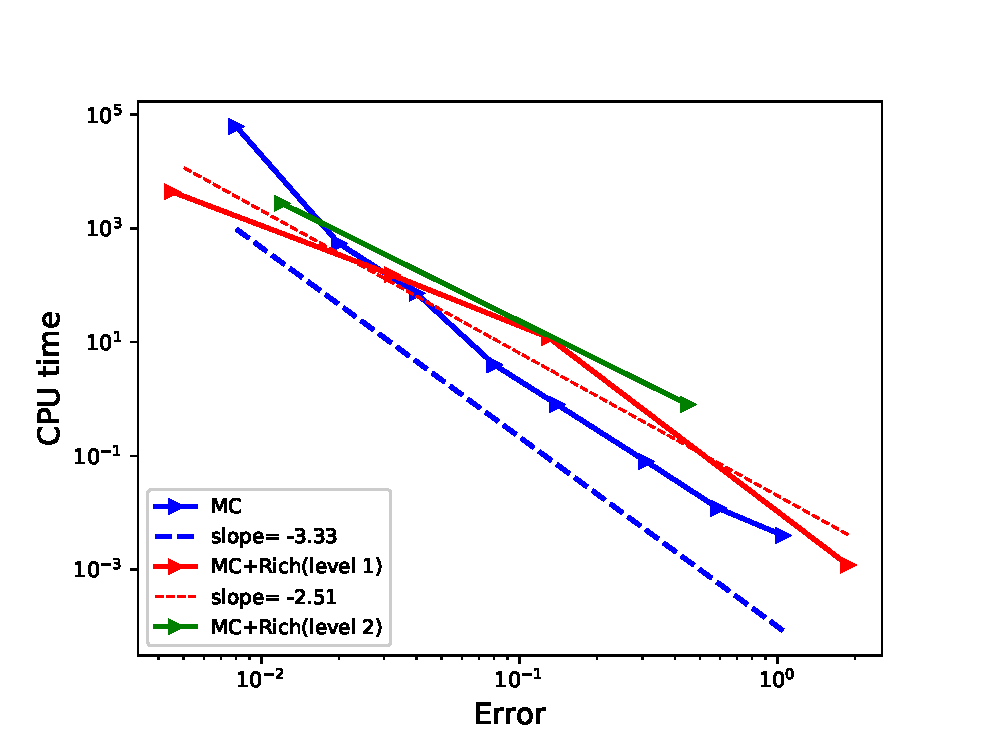
\includegraphics[width=0.9\textwidth]{./rBergomi_Complexity_rates/set2/error_vs_time_set2_MC_comparison}
		\caption{}
	\end{subfigure}
	\begin{subfigure}{0.495\textwidth}
		\centering
		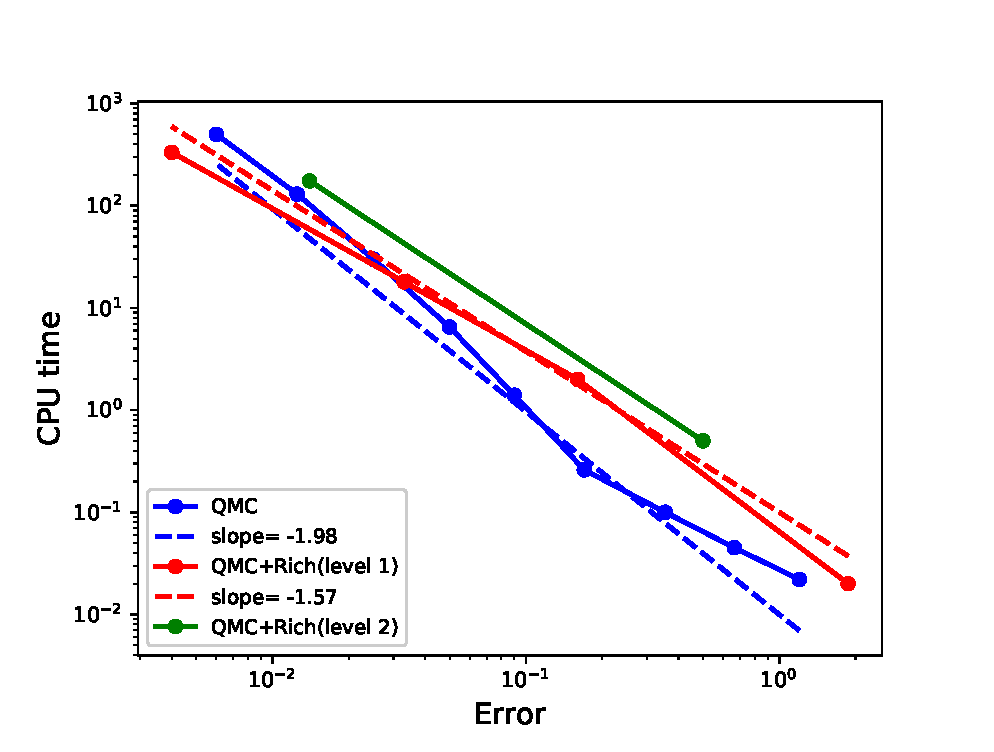
\includegraphics[width=0.9\textwidth]{./rBergomi_Complexity_rates/set2/error_vs_time_set2_QMC_comparison}
		\caption{}
	\end{subfigure}
	\begin{subfigure}{0.5\textwidth}
		\centering
		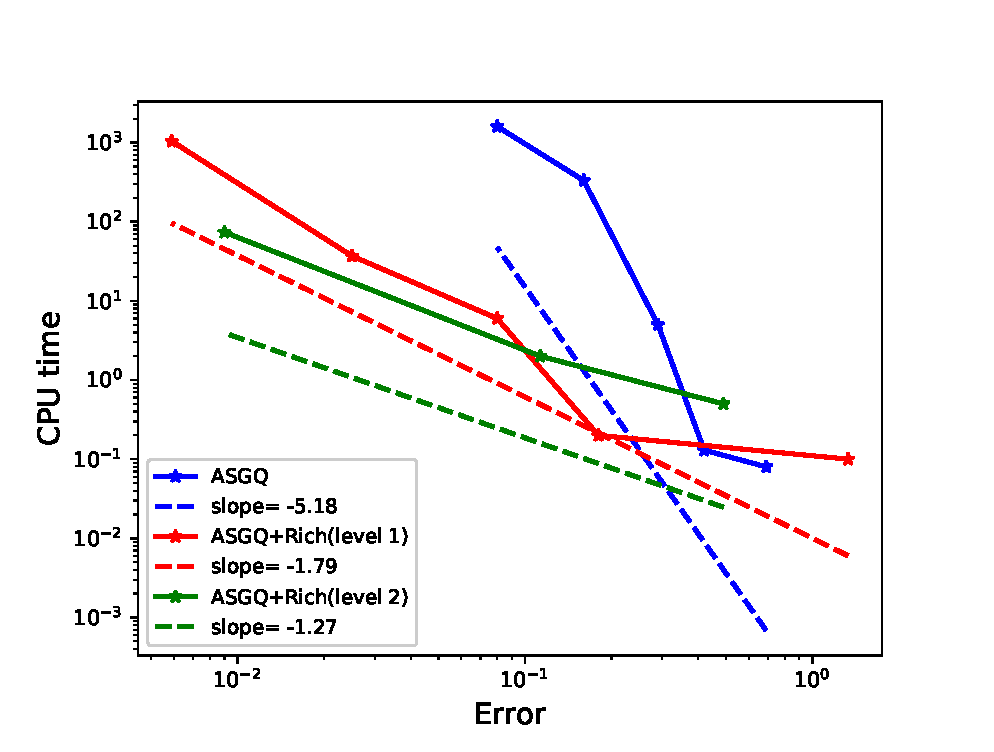
\includegraphics[width=0.9\textwidth]{./rBergomi_Complexity_rates/set2/error_vs_time_set2_MISC_comparison}
		\caption{}
	\end{subfigure}%%
	\caption{Comparing the numerical complexity of the different  methods with the different configurations in terms of the level of Richardson extrapolation,  for the case of \red{parameter set $1$ in Table \ref{table:Reference solution, using MC with $500$ time steps, of Call option price under rBergomi model, for different parameter constellation.}}. a) \red{MC methods}. b) \red{QMC methods}. d) \red{ASGQ methods}. }
	\label{fig: Comparing the numerical complexity of the different  methods with the different configurations}
\end{figure}
\section*{Comparing the Numerical Complexity of the Best Configurations}

\begin{figure}[h!]
	\centering
	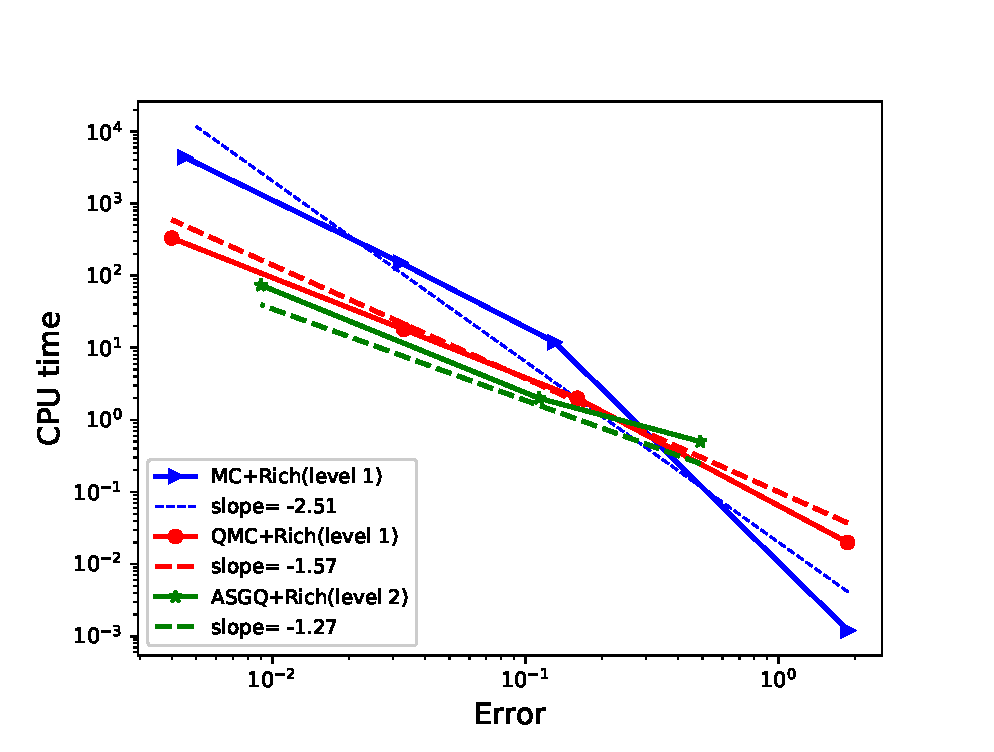
\includegraphics[width=0.7\linewidth]{./rBergomi_Complexity_rates/set2/error_vs_time_set2_full_comparison}
	\caption{Computational work comparison for the different methods \red{with the best configurations concluded from Figure \ref{fig: Comparing the numerical complexity of the different  methods with the different configurations}}, for the case of \red{parameter set $1$ in Table \ref{table:Reference solution, using MC with $500$ time steps, of Call option price under rBergomi model, for different parameter constellation.}}.}	\label{fig:Complexity plot for  MISC for Case set $2$ parameters, comparison}
\end{figure}

%\section*{Conclusions}
%\begin{itemize}
%\item 
%\end{itemize}
%-------------

\section*{Acknowledgements}
C. Bayer gratefully acknowledges support from the German Research Foundation (DFG, grant BA5484/1). This work was supported by the KAUST Office of Sponsored Research (OSR) under Award No. URF/1/2584-01-01 and the Alexander von Humboldt Foundation. C. Ben Hammouda and R. Tempone are members of the KAUST SRI Center for Uncertainty Quantification. 

\footnotesize
\bibliographystyle{abbrv}
\bibliography{smoothing_rBergomi}

\end{multicols}
\end{document}
 